%%%%% TITLE OF MAIN DOCUMENT %%%%%
%% NUMBER AND TITLE OF SECTION %%


%Some sample text to be displayed above the first subsection

%\subsection{Prinzip}

%Ein Zyklotron besteht aus Zwei hohlen, halbzylindrischen und Duanden an denen eine Spannung mit unterschiedlichem Vorzeichen anliegt, und darüber bzw. darunter liegende Magneten, die ein homogenes Magnetfeld erzeugen. Zudem gibt es einen Einlass und einen Auslass für Teilchen.

%\begin{wrapfigure}{r}{0.4\textwidth} \label{Zyklo}
%
%	\vspace{-10pt}
%	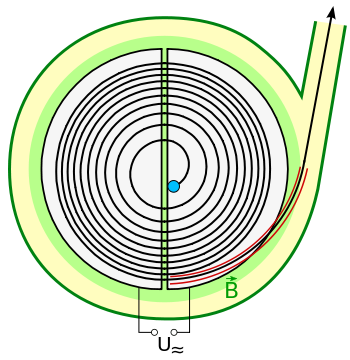
\includegraphics[width=0.35\textwidth]{Zyklotron_Prinzipskizze02.png}
%	\vspace{-13pt}
%	\caption{Prinzipskizze eines Zyklotrons}
%	\vspace{-5pt}	
%	
%\end{wrapfigure}

%\subsubsection{Anwendung}

% Some Formula:

%\begin{equation}
%	x= \frac{y \cdot 13 \pi z}
%			{\cos \alpha}
%\end{equation}

%%%%%%%%%%%%%%%%%%%%%%%
% Eigentlicher Beginn %
%%%%%%%%%%%%%%%%%%%%%%%

\subsection{Definition}

Lange Spulen sind gerade und deren Länge ist größer als deren Durchmesser.


\subsection{Gesetze}

Die magnetische Flussdichte im Inneren einer stromdurchflossenen Spule in definiert als:

\begin{equation} \label{eq:MaFluss}
	B = 	\mu_0 \mu_r \cdot N \cdot \frac{I}{l}
\end{equation}